
%\addcontentsline{toc}{chapter}{\bf cHA}

%\begin{center}
%	{\Large{\bf{CHAPTER 1}}}\\
%\end{center}

%\addcontentsline{toc}{chapter}{\bf Acknowledgements}
%\addcontentsline{toc}{chapter}{\bf ACKNOWLEDGEMENTS}

%\begin{center}
%	{\Large{\bf{CHAPTER 1}}}\\
%\end{center}

\chapter{MOTIVATION/INTRODUCTION}

\section{{\bf{Context/Rationale/Background}}}
{\bf\color{red}In this section, the author(s) shall discuss the  historical background related to the work along with the introduction of the topic in brief.}
\begin{figure}[h]
	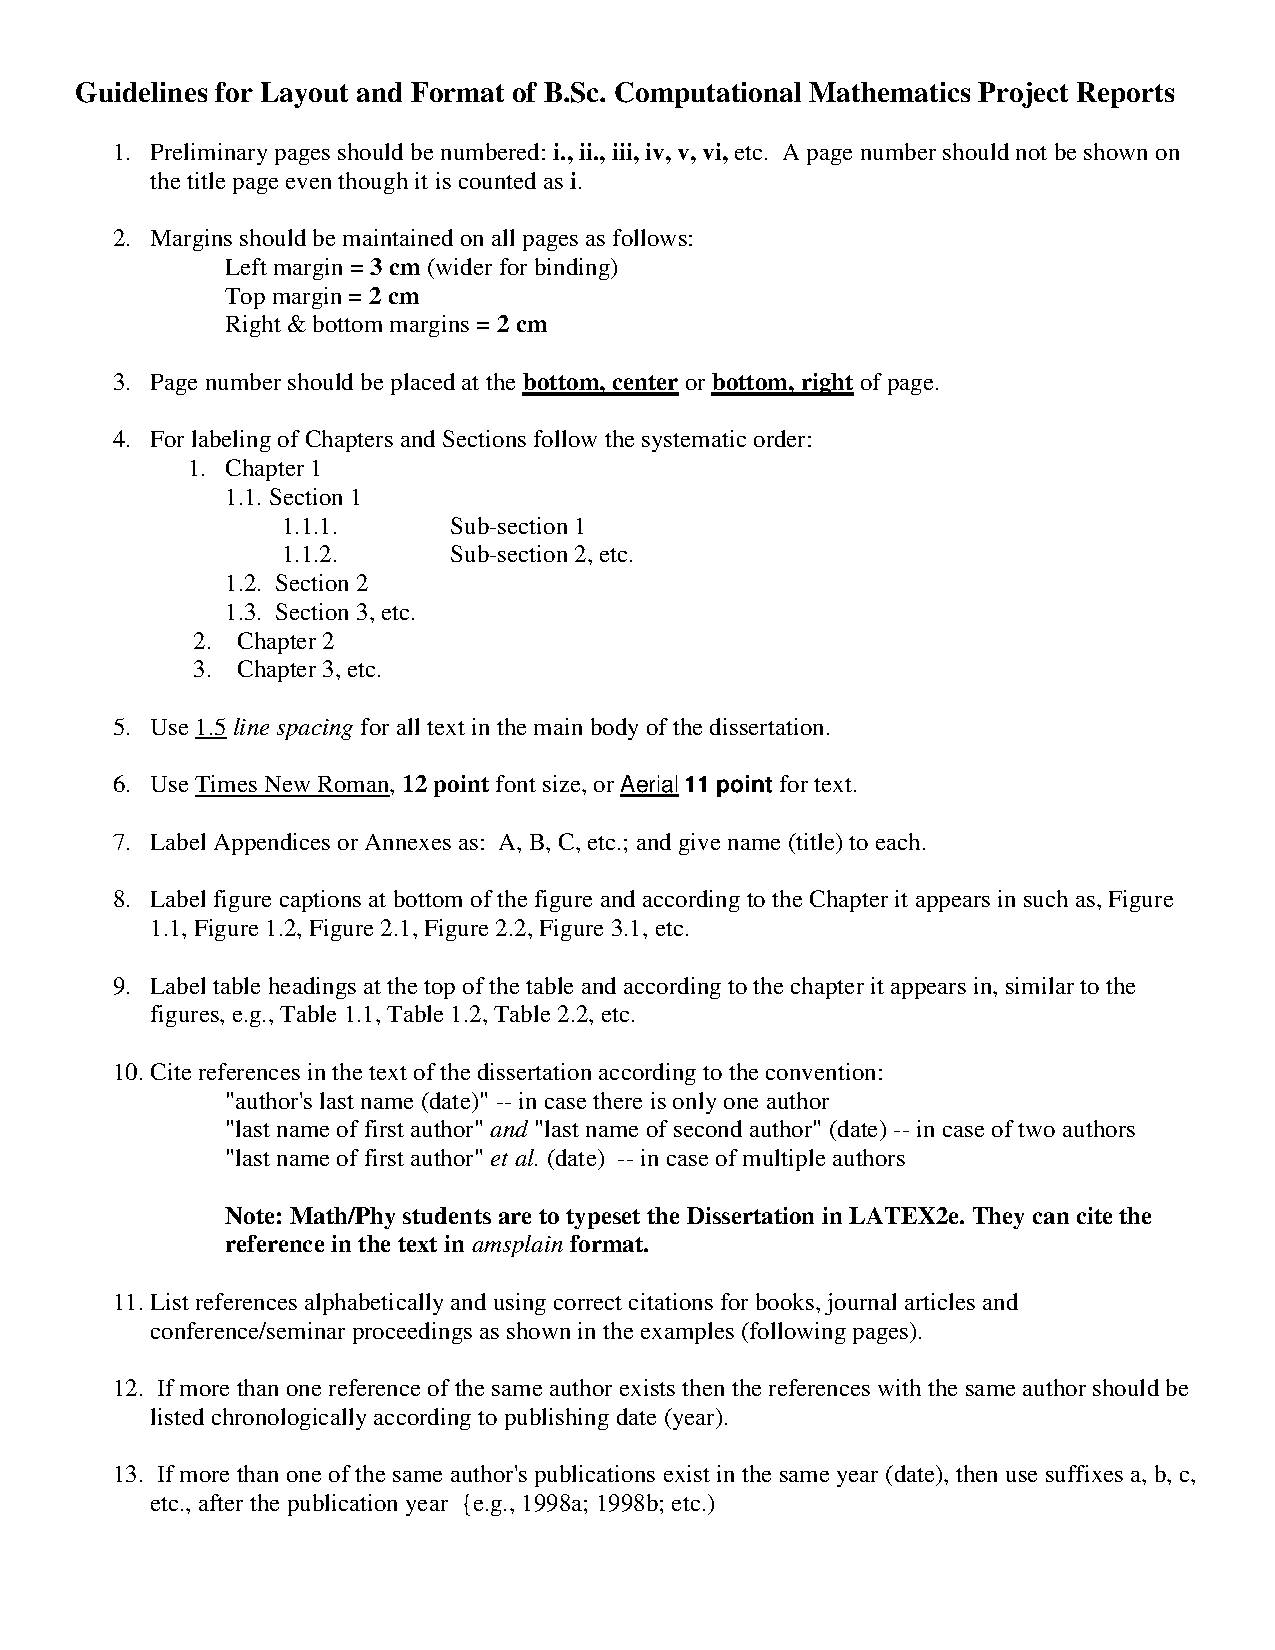
\includegraphics[scale=0.5]{figures/layout.pdf}
\end{figure}




\subsection{\bf The Layout of the  SubSection of the Project Report}
Your first subsection of Section 1 of Chapter 1. \\
{\color{blue} Typeset the following commands to compile the format designed Project report guideline}
%%%%%%%%%%%%%%%%%%%
\begin{verbatim}
\documentclass[a4paper,12pt]{report}    % Document Class
% % % % % % % % % % % % % % % % % % % % % % % % % % % % % % % % %
% % % % PACKAGES
% % % % % % % % % % % % % % % % % % % % % % % % % % % % % % % % %
\linespread{1.5}                    % For line spacing
\usepackage{amssymb}                % For AMS symbol
\usepackage{amsmath}                % This is useful for the matrix 
\usepackage{verbatim}               % For comments in paragraph
\usepackage{graphicx}               % For imbeding graph
\usepackage{color}                  % Color for the text
\usepackage{makeidx}
\usepackage{url}
\usepackage{sectsty}
\chapterfont{\centering}

% % % % % % % % % % % % % % % % % % % % % % %
% % % % FOR ADJUSTMENT OF PAGES
% % % % % % % % % % % % % % % % % % % % % % %
\usepackage[top=2cm, bottom=2cm, left=3cm, right=2cm]{geometry}

% % % % % % % % % % % % % % % % % % % % % % % %
% % % % FOR SHORTCUT USE
% % % % % % % % % % % % % % % % % % % % % % % %
\newtheorem{df}{Definition} % For definition
\newtheorem{exm}{Example}   % For Example
\newtheorem{exe}{Exercise}  % For Exercise
\newtheorem{prob}{Problem}  % For Problem
\newtheorem{task}{TASK}     % For Task
\newtheorem{thm}{Theorem}   % For Theorem
% % % % % % % % % % % % % % % % % % % % % % % % %
\renewcommand{\chaptername}{CHAPTER}
\renewcommand{\contentsname}{\centering CONTENTS}
\renewcommand{\listfigurename}{\centering LIST OF FIGURES}
\renewcommand{\listtablename}{\centering LIST OF TABLES}

%%%%%%%%%%%%%%%%%%%%%%%%%%%%%%%%%%%%%%%%%%%%%%%%%%%%%%%
\pagestyle{plain}
%==================================================================
\begin{document}
% % % % % % % % % % % % %
\pagenumbering{roman}
%===================================================================
%   Begin your document hereafter
%=====================================================================


{\large
\begin{center}
{\color{red}{\bf{Title: A \LaTeXe template to Typeset Your Dissertation}}}\\
\end{center}


\vspace{0.8cm}

{\normalsize
\begin{center}
A DISSERTATION\\

\vspace{0.5cm}
SUBMITTED IN PARTIAL FULFILLMENT OF THE REQUIREMENTS FOR\\
THE DOCTOR OF PHILOSOPHY (PhD) DEGREE\\
IN MATHEMATICS

\vspace{2cm}

BY
\end{center}


\begin{center}
{\color{red} {STUDENT NAME, PREVIOUS DEGREE}}
\end{center}

\vspace{1.5cm}

\begin{figure}[htpb]
\centering

\includegraphics[height=4.5cm,width=4.5cm]{photos/kulogo}
\end{figure}


\vspace{2cm}
{\normalsize
\begin{center}
%DEPARTMENT OF NATURAL SCIENCES (MATHEMATICS)\\
SCHOOL OF SCIENCE\\
KATHMANDU UNIVERSITY\\
DHULIKHEL, NEPAL\\
\end{center}
}

\begin{center}
{\color{red} MONTH AND YEAR OF COMPLETION}
\end{center}
}
}
\thispagestyle{empty}	% No numbering in this page
%===================================================================
\newpage
\input{Dedication}

\newpage
\input{Student_declaration}

\newpage



%\addcontentsline{toc}{chapter}{\bf Certification}
\addcontentsline{toc}{chapter}{\bf CERTIFICATION}

\begin{center}
	{\Large{\bf{ CERTIFICATION}}}
\end{center}


\noindent
This project entitled "Modeling and use of FEM on static structure" is carried out  under my supervision for the specified entire period satisfactorily, and is hereby certified as a work done by following students
\begin{itemize}
\item[1.] Samrajya Raj Acharya (Exam Roll No.)
\item[2.] Bishesh Kafle (Exam Roll No.)
\item[3.] Priyanka Panta (Exam Roll No.)
\item[4.] Mukesh Tiwari (Exam Roll No.)
\end{itemize}
 in partial fulfillment of the requirements for the degree of B.Sc. in Computational Mathematics, Department of Mathematics, Kathmandu University, Dhulikhel, Nepal.

\vspace{1.0cm}

\noindent
--------------------------\\
{\bf Dr. Gokul KC}\\
Assistant Professor \\
Department of Mathematics,\\
School of Science, Kathmandu University,\\
Dhulikhel, Kavre, Nepal\\
Date:\today

\vspace{1cm}

\noindent
{\bf APPROVED BY:}\\
I hereby declare that the candidate qualifies to submit this  report of the  Math Project (MATH-252) to the Department of Mathematics. 



\vspace{2cm}

\noindent
-----------------------------\\
Head of the Department\\
Department of Natural Sciences\\
School of Science\\
Kathmandu University\\
Date:\today
  

\newpage
\input{ack}

\newpage
\input{abs}

% ===================================================================

\tableofcontents

\listoffigures
\addcontentsline{toc}{chapter}{LIST OF FIGURES}

\listoftables
\addcontentsline{toc}{chapter}{LIST OF TABLES}

\newpage
\input{param}

% ====================================================================
\newpage
\pagenumbering{arabic}
%\input{chap1}
\include{chap1}

\newpage
\input{chap2}

\newpage
\include{publ}
%=====================================================================
% For Reference settings
%%%%%%%%%%%%%%%%%%%%%%%%%%%%%%%%%%%%%%%%%%%%%%%%%%%%%%%%%%%%%%%%%%%%%
\renewcommand{\bibname}{\centering REFERENCES}
\bibliographystyle{amsplain}
\addcontentsline{toc}{chapter}{REFERENCES}
\bibliography{bibtex_database/myrefs} % data base
%===================================================================
\end{document}
\end{verbatim}
%%%%%%%%%%%%%%%%%

\subsection{\bf AMS Plain Format for References and Citation in Text}
Your second subsection of Section 1 of Chapter 1.

\noindent
{\color{red}
	Online resource in AMS format as in Doe  \cite{Doe}\\
	Proceeding in AMS format is as in Gokul \cite{Gokul}\\
	PhD Dissertation in AMS format is as in Gurung \cite{db1}.\\
	Book in AMS format is as in Kopka and Daly \cite{HK}\\
	Article in AMS format is as in Roy et al. \cite{db3}.\\
	
}
--------------------------------------------------------------------------------------------------------------------
\begin{itemize}
	\item
	{\bf If your citation of an article/book contains one or two authors, then {\color{red} {cite it writing authors surname}}. For example as shown in {\color{blue}{Kopka and Daly \cite{HK}}}}.
	\item
	{\bf If your citation of an article/book contains more than two authors, then {\color{red}{cite it writing first author surname followed by et al.}} . For example as shown in {\color{blue}{Roy et al. \cite{db3}}}}.
\end{itemize}

\noindent
{\color{blue} \bf The current use of reference style is {\color{red} amsplain} in KU M.Phil and PhD Dissertation guideline. The other styles used in \LaTeX package are abbrv, acm, alpha, plain, amsalpha, apalike, ieeetr, siam, unstr.}



\section{{\bf{Objectives}}}
{\bf\color{red}In this section, the author(s) should enlist to sets of objectives
\begin{enumerate}
 \item  Specific objectives 
 \item General objectives 
\end{enumerate}
}

\section{\bf Significance/Scope}
{\bf\color{red}In this section, the author(s) shall discuss the relevance and the underlying problems that may rise to the need to do this project/work.}
\begin{table}[htpb]
\caption{Name and Notation.}
\begin{center}
\begin{tabular}{|c|c|c|}\hline
Category & Intuitive meaning & Typical element \\ \hline
                                                    \hline
$\mathit{Nml}$ & numerals & $N$ \\ \hline
$\mathit{UnOps}$ & unary operators & $\alpha$ \\ \hline
$\mathit{BinOps}$ & binary operators & $\omega$ \\ \hline
$\mathit{Ide}$ & identifiers & $I$ \\ \hline
$\mathit{Exp}$ & expressions & $E$ \\ \hline
$\mathit{Cmd}$ & commands & $C$ \\ \hline
\end{tabular}
\end{center}
\end{table}

\section{\bf Limitations}
{\bf\color{red}In this section, the author(s) should enlist or elaborate the possible limitations of the project or the difficulty foreseeable during the work.}
\begin{figure}[htpb]
\begin{center}
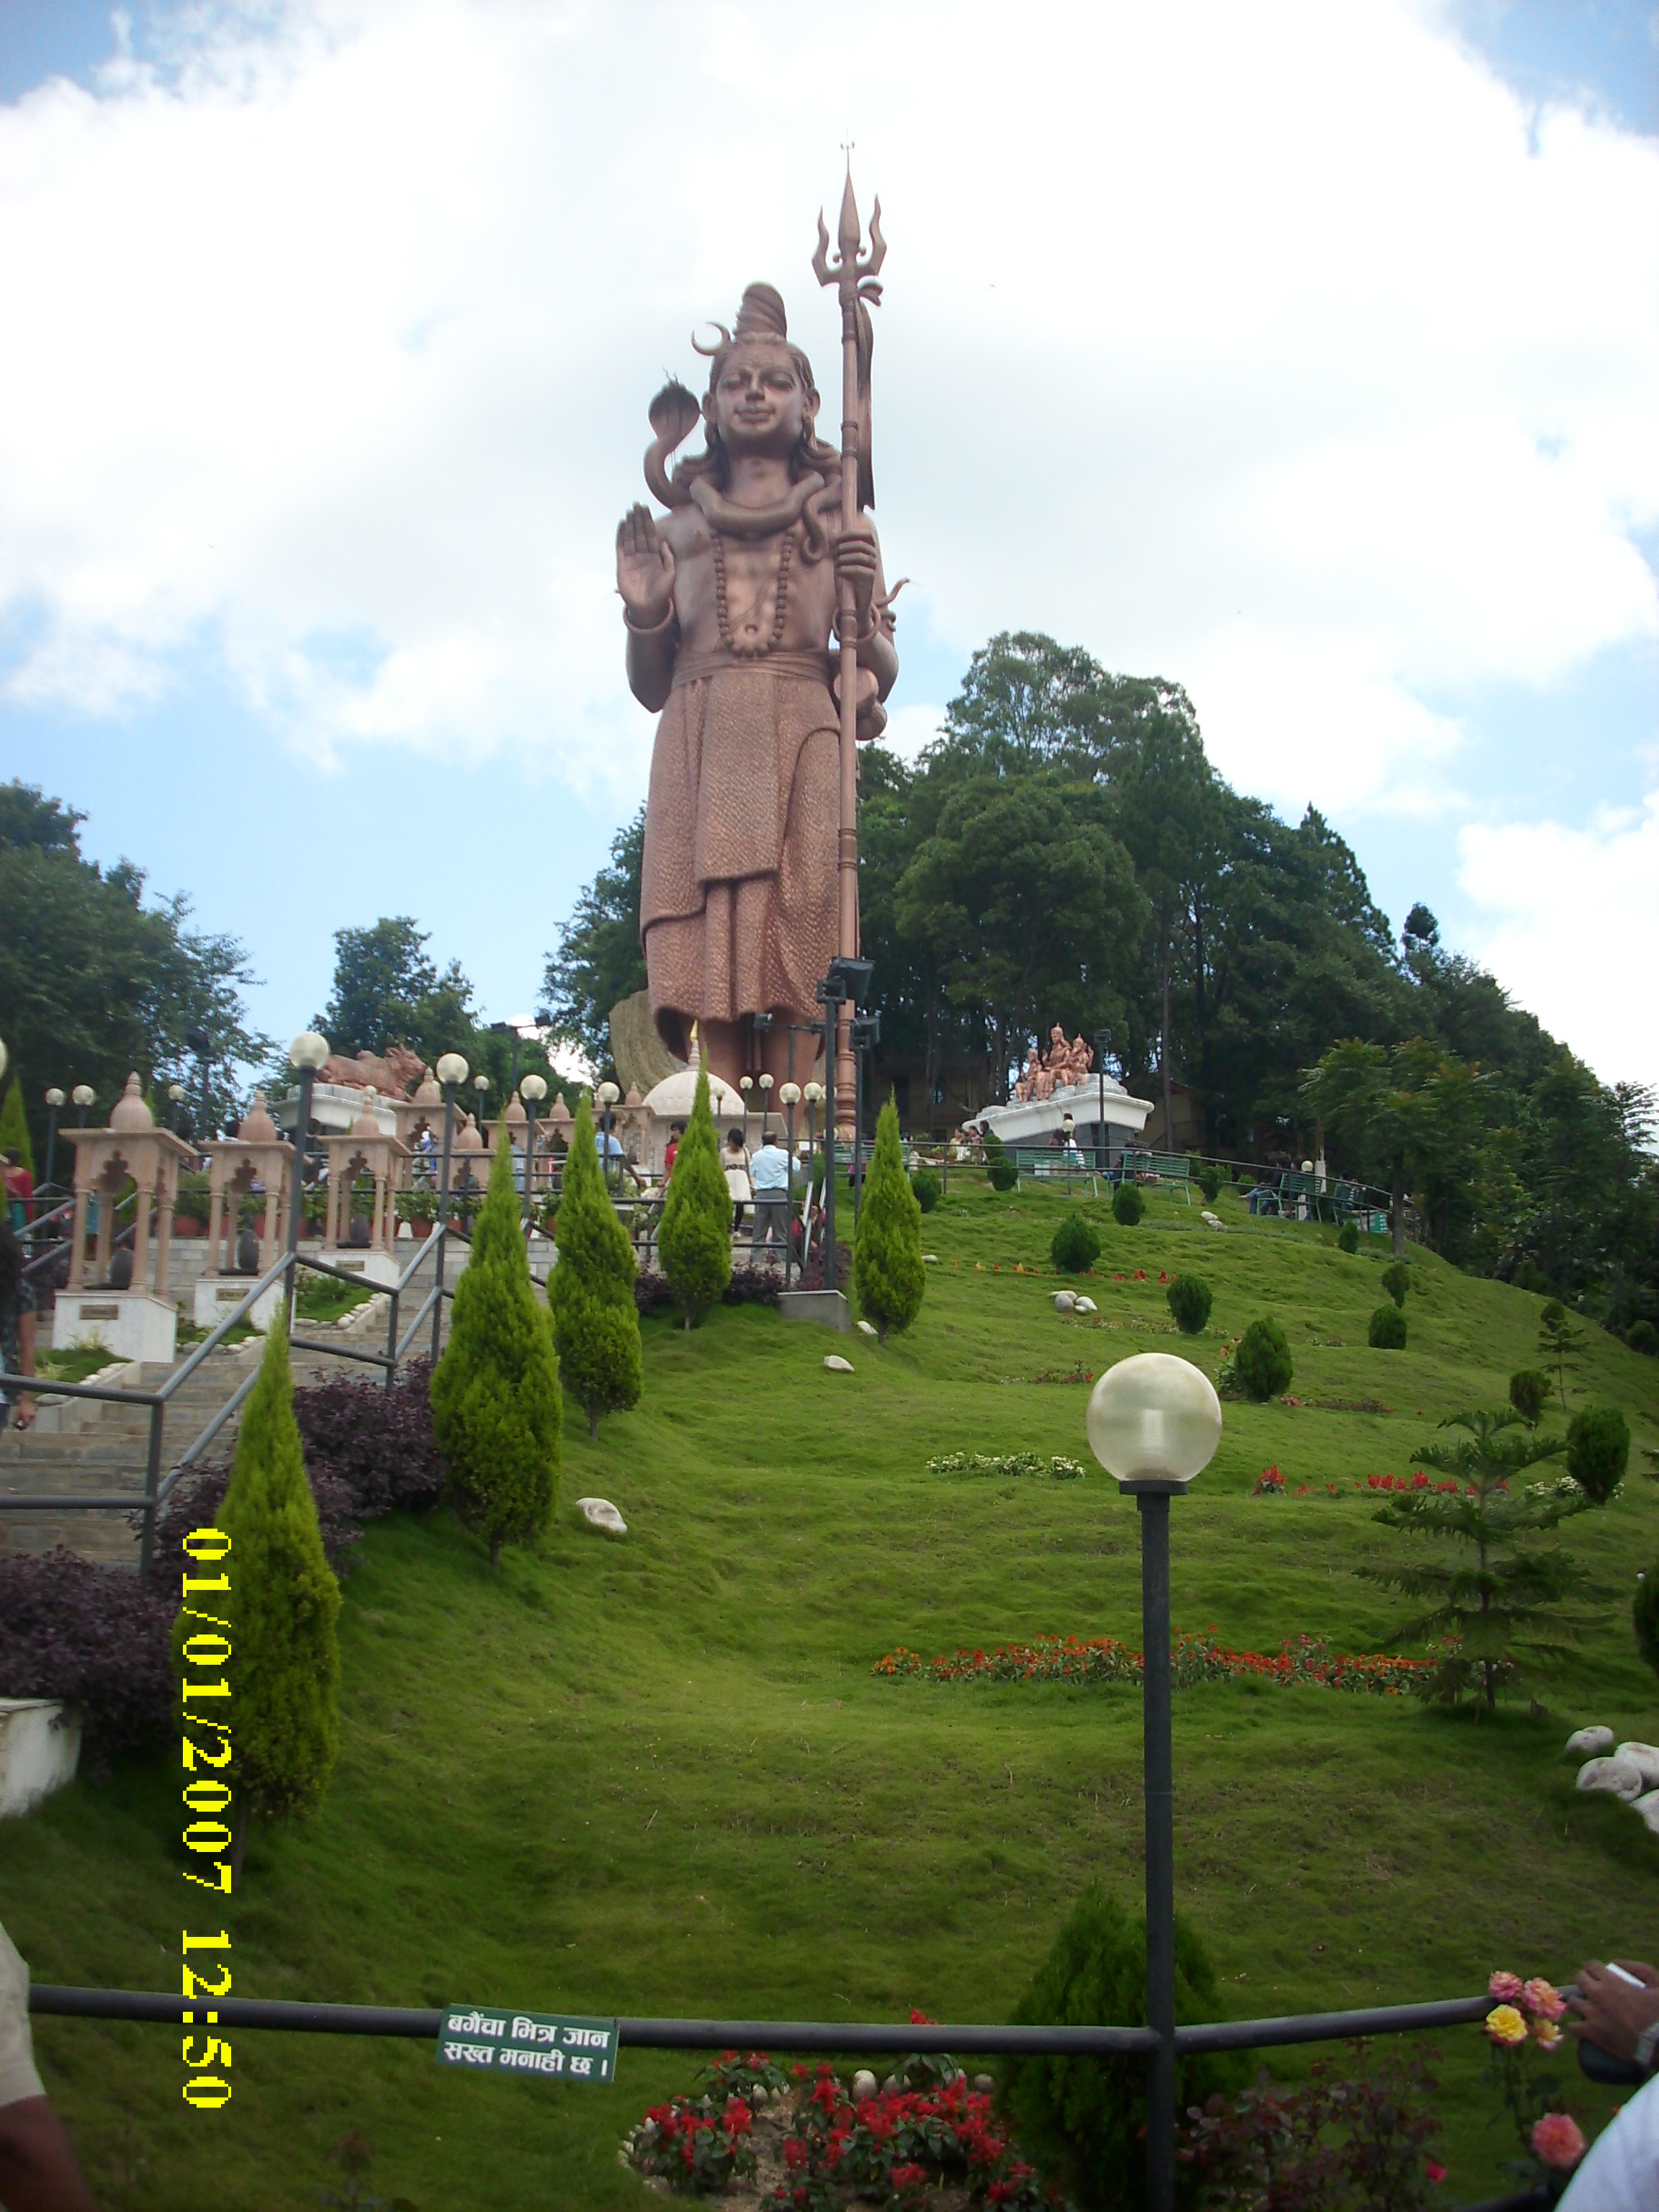
\includegraphics[height=8cm, width=8cm]{figures/sanga.JPG}
\caption{Shiva Statue Sangha}
\label{fig1.6}
\end{center}
\end{figure}
